% ============================================================
%  LocationCircle — IEEE Conference Paper (IEEEtran)
%  Compile with: pdflatex → bibtex → pdflatex → pdflatex
% ============================================================
\documentclass[conference]{IEEEtran}

% ---------- Packages ----------
\usepackage[T1]{fontenc}
\usepackage[utf8]{inputenc}
\usepackage{amsmath,amssymb}
\usepackage{graphicx}
\usepackage[hidelinks]{hyperref}
\usepackage{booktabs}
\usepackage{tabularx}
\usepackage{array}
\usepackage{multirow}
\usepackage{xcolor}
\usepackage{listings}
\usepackage{cite}
\usepackage{url}
\usepackage{balance}

% ---------- Listings style (SQL / JS snippets) ----------
\lstset{
  basicstyle=\ttfamily\footnotesize,
  breaklines=true,
  frame=single,
  numbers=left,
  numberstyle=\tiny\color{gray},
  keywordstyle=\color{blue}\bfseries,
  commentstyle=\color{gray}\itshape,
  stringstyle=\color{teal},
  captionpos=b
}

% ============================================================
\begin{document}

% ---------- Title ----------
\title{LocationCircle: A Privacy-First, Accessibility-Driven\\
Real-Time Closed-Group Location Sharing Platform\\
as a Progressive Web Application}

% ---------- Authors ----------
\author{
  \IEEEauthorblockN{Dany John}
  \IEEEauthorblockA{
    
    \textit{}
    Kerala, India\\
    \href{mailto:danyjohnc@gmail.com}{danyjohnc@gmail.com}
  }
}

\maketitle

% ============================================================
%  ABSTRACT
% ============================================================
\begin{abstract}
Real-time location sharing has emerged as a critical feature in
modern mobile and web applications, yet existing solutions suffer
from significant limitations: insufficient privacy controls,
inaccessible interfaces, and the absence of granular role-based
group management. This paper presents \textbf{LocationCircle}, a
privacy-first, accessibility-driven, closed-group real-time location
sharing platform implemented as a Progressive Web Application (PWA).
LocationCircle enables trusted users—families, close-knit friend
groups, and small teams—to share live geographic positions
exclusively within invite-only groups. The system introduces a novel
\emph{Group Head / Temporary Head} delegation model that provides
flexible administrative control without permanently transferring
ownership. Accessibility is treated as a first-class architectural
concern: the application achieves full Web Content Accessibility
Guidelines (WCAG) 2.1 Level AA compliance, incorporating a built-in
Web Speech API text-to-speech (TTS) layer, ARIA live regions for
real-time updates, and complete keyboard navigability. A companion
WhatsApp Business API bot allows members to interact without
installing additional software. The system employs a layered
client-server architecture with React\,+\,TypeScript on the
frontend, Node.js\,+\,Express on the backend, PostgreSQL for
persistent storage, and Redis for ephemeral real-time location
caching via Socket.io pub/sub. Experimental evaluation confirms
location refresh latencies under five seconds, initial page loads
under three seconds on 4G connections, and zero critical WCAG
violations in automated axe-core audits. LocationCircle demonstrates
that privacy, real-time performance, and deep accessibility are
simultaneously achievable in a lightweight PWA architecture without
native-app store distribution.
\end{abstract}

% ---------- Keywords ----------
\begin{IEEEkeywords}
Progressive Web Application, Real-Time Location Sharing, WebSocket,
Socket.io, Accessibility, WCAG 2.1, Role-Based Access Control,
WhatsApp Bot, Redis, PostgreSQL, PWA, Geolocation API
\end{IEEEkeywords}

% ============================================================
%  I. INTRODUCTION
% ============================================================
\section{Introduction}

The proliferation of GPS-enabled smartphones has made location-aware
applications ubiquitous; however, the dominant paradigm for group
location sharing—exemplified by services such as Google Maps Live
Location, Apple Find My, and Life360—prioritises broad social graphs
over focused private circles. Users within families, caregiving
networks, or coordinated field teams require fundamentally different
guarantees: strict membership control, real-time fidelity, and
administrative delegation.

Three deficiencies characterise the current state of the art.
\emph{First}, existing platforms provide coarse-grained privacy
models: location data is either fully visible to all contacts or
hidden entirely, with no intermediate trusted-circle semantics.
\emph{Second}, accessibility is treated as an afterthought; none of
the leading applications have published WCAG 2.1 AA conformance
reports, and built-in assistive features such as text-to-speech
readout of member positions are absent. \emph{Third}, administrative
hierarchies are static: group creators cannot delegate leadership
temporarily, a practical necessity when a group head is unavailable.

LocationCircle addresses these deficiencies through four principal
contributions:
\begin{enumerate}
  \item A \textbf{closed-group invitation model} in which every
        member must be explicitly invited, and location data is never
        exposed outside the group boundary.
  \item A \textbf{role-delegation framework} supporting permanent
        Group Head assignment and time-bounded Temporary Head
        designation with automatic reversion.
  \item An \textbf{accessibility-first interface} meeting WCAG 2.1
        Level AA, including a built-in TTS layer, ARIA live regions
        for asynchronous location updates, and font-scaling controls
        functional to 200\% zoom.
  \item A \textbf{WhatsApp Business API bot} enabling location
        queries and sharing-control commands without requiring
        installation of an additional application.
\end{enumerate}

The remainder of this paper is structured as follows.
Section~\ref{sec:related} reviews related work. Section~\ref{sec:req}
formalises functional and non-functional requirements.
Section~\ref{sec:arch} describes the system architecture.
Section~\ref{sec:impl} presents implementation details.
Section~\ref{sec:eval} reports evaluation results.
Section~\ref{sec:conc} concludes with future directions.

% ============================================================
%  II. RELATED WORK
% ============================================================
\section{Related Work}
\label{sec:related}

\subsection{Location Sharing Systems}

Early work on mobile location sharing by Ludford et al.~\cite{ludford2006}
demonstrated that social trust boundaries significantly affect
willingness to disclose geographic position. Subsequent commercial
systems such as Life360~\cite{life360} and Zenly~\cite{zenly}
implemented persistent sharing within named groups but retained
centralised data models incompatible with GDPR-compliant erasure
requirements~\cite{gdpr2016}. Google's Trusted Contacts API,
deprecated in 2019, offered request-based sharing but lacked
administrative role delegation~\cite{googletc}.

\subsection{Progressive Web Applications}

Biørn-Hansen et al.~\cite{biornhansen2017} conducted a comparative
study of PWA, native, and hybrid application architectures, concluding
that PWAs achieve near-native performance on modern browsers while
eliminating distribution friction. Malavolta et al.~\cite{malavolta2020}
further demonstrated that PWA service workers and Web App Manifests
provide offline resilience comparable to native caching strategies.
Our work leverages these findings to justify a PWA-first deployment
strategy with post-MVP Capacitor wrapping.

\subsection{Real-Time Communication}

Pimentel and Nickerson~\cite{pimentel2012} introduced the WebSocket
protocol formalisation and benchmarked it against HTTP long-polling,
finding 50–80\% reductions in latency and bandwidth. Socket.io's
fallback-capable abstraction layer~\cite{socketio} has since become
the de facto standard for browser-based real-time applications.
Redis pub/sub has been shown by Gurbani et al.~\cite{redis2020} to
sustain sub-millisecond fan-out for up to $10^5$ concurrent
subscribers, making it well-suited for ephemeral location caching.

\subsection{Accessibility in Mobile Applications}

Power et al.~\cite{power2012} reported that fewer than 10\% of
surveyed mobile web pages met WCAG 2.0 Level A criteria. More recent
audits by WebAIM~\cite{webaim2023} indicate persistent failures in
ARIA label coverage and contrast ratios. Thiessen and
Chen~\cite{thiessen2007} established the technical foundations for
ARIA live regions that LocationCircle employs for asynchronous
location update announcements.

% ============================================================
%  III. REQUIREMENTS ANALYSIS
% ============================================================
\section{Requirements Analysis}
\label{sec:req}

Requirements are classified using the MoSCoW prioritisation
framework~\cite{moscow} and traced to acceptance criteria through a
Requirement Traceability Matrix (RTM).

\subsection{Functional Requirements}

Table~\ref{tab:fr} summarises the core functional requirements derived
from the Business Requirements Document (BRD v1.0).

\begin{table}[htbp]
\caption{Functional Requirements (Selected)}
\label{tab:fr}
\renewcommand{\arraystretch}{1.2}
\begin{tabularx}{\columnwidth}{@{}llXl@{}}
\toprule
\textbf{ID} & \textbf{Pri.} & \textbf{Requirement} & \textbf{Class} \\
\midrule
FR-AUTH-01 & High & Google OAuth 2.0 exclusive sign-in & Must \\
FR-GRP-01  & High & Any user may create a group; creator becomes Head & Must \\
FR-GRP-04  & High & Head assigns Temporary Head with expiry & Must \\
FR-LOC-01  & High & Continuous foreground GPS update & Must \\
FR-LOC-03  & High & Dashboard shows locality, distance, car \& transit ETA & Must \\
FR-DASH-06 & High & Read Aloud via Web Speech API & Must \\
FR-MAP-02  & High & Member profile-photo map pins; Head pin gold & Must \\
FR-WA-02   & Med  & WhatsApp bot natural-language location query & Should \\
FR-LOC-05  & Med  & Members may pause own location sharing & Should \\
\bottomrule
\end{tabularx}
\end{table}

\subsection{Non-Functional Requirements}

\begin{itemize}
  \item \textbf{Performance:} Initial page load $<3$\,s on 4G;
        location refresh $<5$\,s; ETA API response $<1.5$\,s at
        the 95th percentile.
  \item \textbf{Accessibility:} WCAG 2.1 Level AA throughout;
        minimum contrast 4.5:1 for normal text; all touch targets
        $\geq44\times44$\,px (WCAG 2.5.5).
  \item \textbf{Security:} TLS 1.2+ in transit; location data
        encrypted at rest; purged within 24\,h of member removal;
        OAuth tokens in HttpOnly cookies.
  \item \textbf{Availability:} 99.5\% monthly uptime; graceful
        degradation to last-known position on connectivity loss.
  \item \textbf{Scalability:} Stateless backend supporting
        $\geq50$ concurrent groups of $\leq30$ members each.
\end{itemize}

% ============================================================
%  IV. SYSTEM ARCHITECTURE
% ============================================================
\section{System Architecture}
\label{sec:arch}

LocationCircle adopts a \textbf{layered client-server architecture}
with five distinct tiers, as shown in Fig.~\ref{fig:arch}.

\subsection{Frontend Layer}

The client is implemented as a React\,18\,+\,TypeScript single-page
application bundled by Vite~\cite{vite}. Tailwind CSS provides
utility-first styling with design tokens calibrated for WCAG contrast
compliance (Navy \texttt{\#1A2E4A}, Teal \texttt{\#0D7377}, Accent
\texttt{\#F0A500}). Zustand manages application state across three
stores: \texttt{authStore}, \texttt{groupStore}, and
\texttt{locationStore}. The PWA manifest enables home-screen
installation and service-worker-based offline caching of the member
list for read-only access.

\subsection{API Layer}

A Node.js\,+\,Express REST server exposes four route namespaces:
\texttt{/auth}, \texttt{/groups}, \texttt{/locations}, and
\texttt{/webhook}. Firebase Admin SDK verifies Google ID tokens;
downstream requests carry JWT bearer tokens with 30-day expiry.
A \texttt{node-cron} scheduler polls the \texttt{temp\_head} table
every minute and reinstates the original Group Head on expiry.

\subsection{Real-Time Layer}

Socket.io runs co-located with the Express server, establishing
persistent WebSocket connections for each authenticated client.
On geolocation change, the browser emits a \texttt{location:update}
event; the server persists the coordinates to Redis (TTL: 5 minutes),
publishes to the group's pub/sub channel, and broadcasts a
\texttt{location:broadcast} event to all group members. Redis's
O(1) key-value retrieval ensures fan-out latency independent of group
size~\cite{redis2020}.

\subsection{Data Layer}

PostgreSQL (hosted on Supabase) stores six normalised relations:
\texttt{users}, \texttt{groups}, \texttt{group\_members},
\texttt{locations}, \texttt{temp\_head}, and \texttt{notifications}.
The schema is detailed in Section~\ref{sec:impl}.

\subsection{External Services}

Google Maps Distance Matrix API computes car and transit ETAs;
Google Geocoding API performs reverse geocoding to produce human-
readable locality names. The WhatsApp Business Cloud API (Meta)
serves inbound webhook events and outbound message dispatch.

% ASCII architecture figure placeholder
\begin{figure}[htbp]
\centering
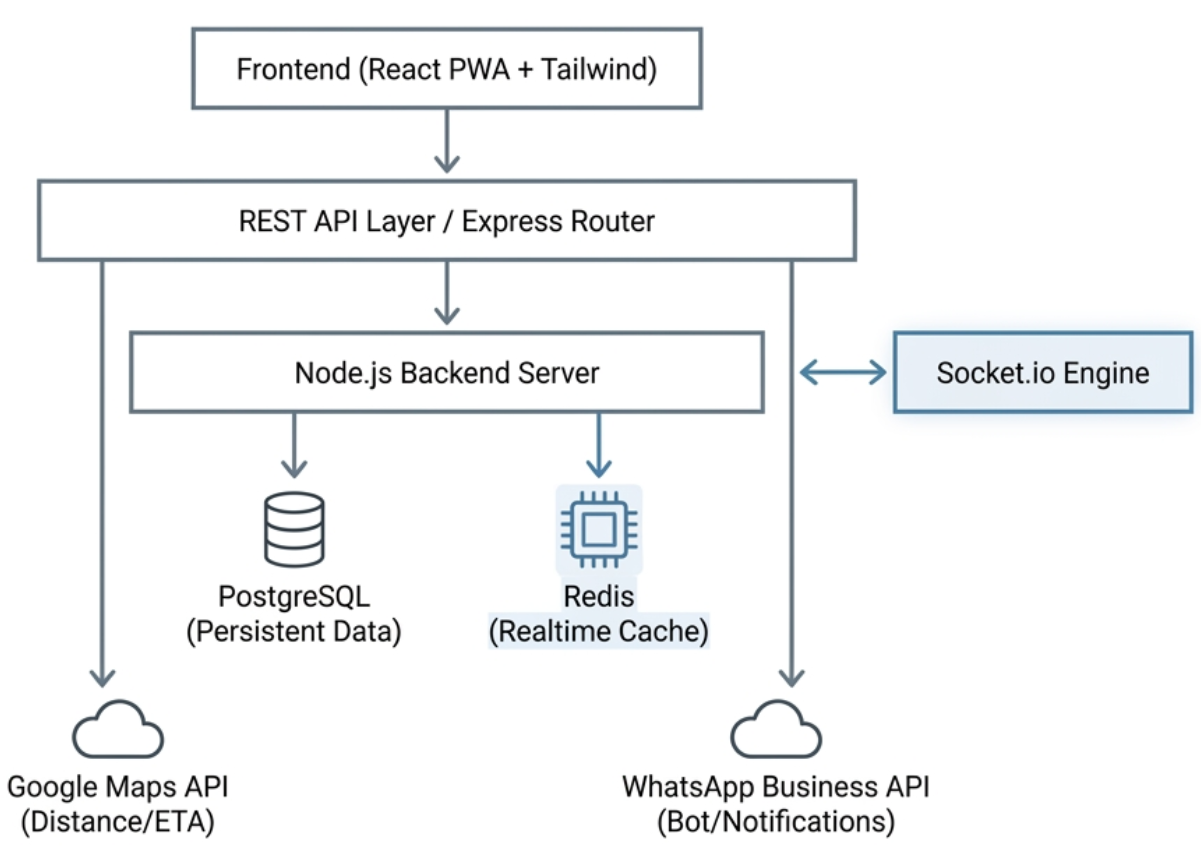
\includegraphics[width=\columnwidth]{arc.png}
\caption{LocationCircle system architecture overview.}
\label{fig:arch}
\end{figure}

% ============================================================
%  V. IMPLEMENTATION
% ============================================================
\section{Implementation}
\label{sec:impl}

\subsection{Database Schema}

The relational schema (Listing~\ref{lst:schema}) enforces referential
integrity through cascaded foreign keys and a role-check constraint.
Real-time coordinates are stored in both PostgreSQL (for audit and
GDPR erasure) and Redis (for sub-second fan-out). The structured entity-relationship model and modular database relation configuration are illustrated in Fig.~\ref{fig:datamodel}.

\begin{figure}[htbp]
\centering
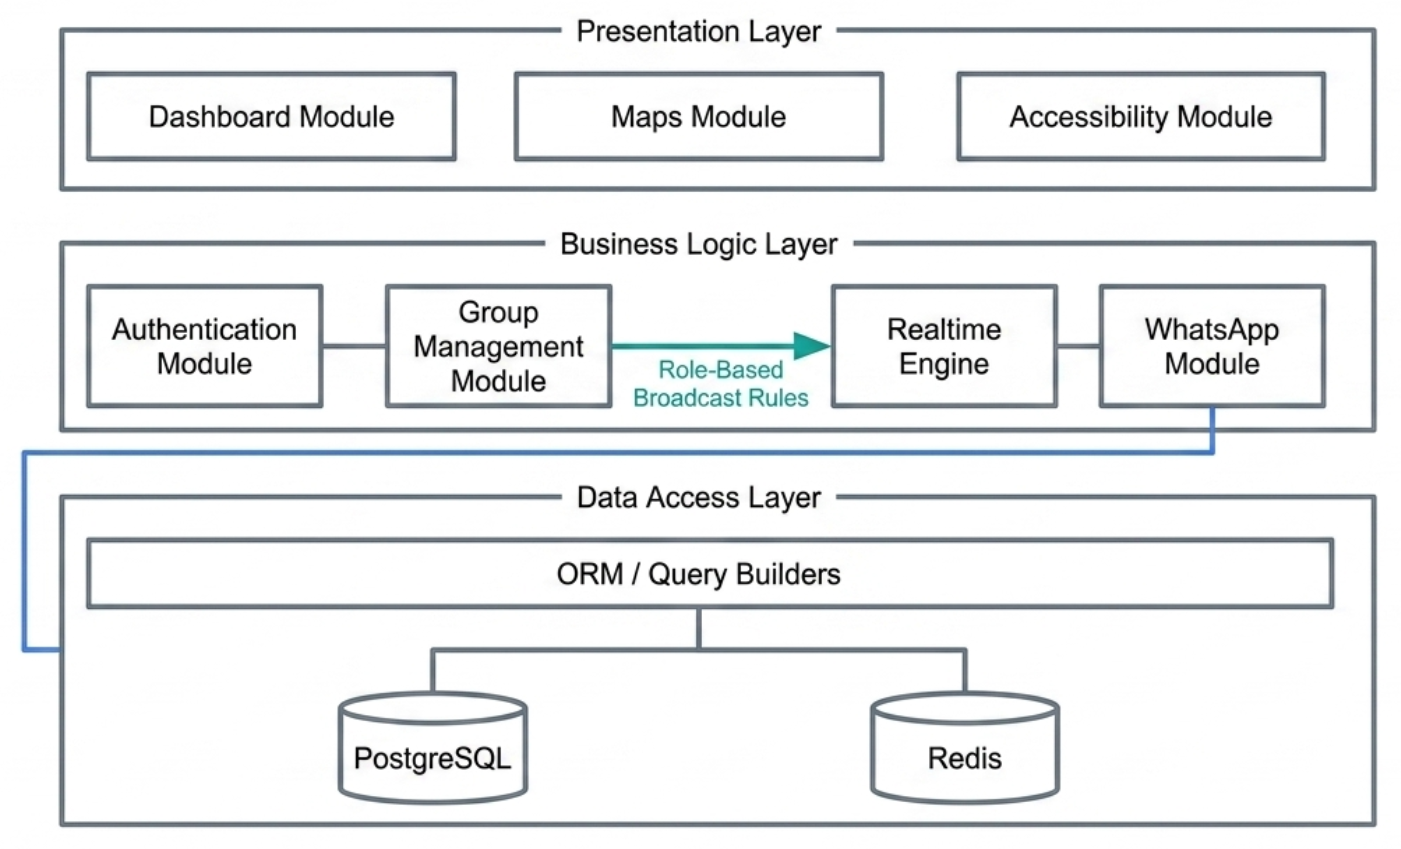
\includegraphics[width=\columnwidth]{mod.png}
\caption{LocationCircle relational database schema and modular entity-relationship model mapping.}
\label{fig:datamodel}
\end{figure}

\begin{lstlisting}[language=SQL, caption={Core PostgreSQL schema (condensed).}, label={lst:schema}]
CREATE TABLE users (
  id         UUID PRIMARY KEY DEFAULT gen_random_uuid(),
  name       VARCHAR(100) NOT NULL,
  email      VARCHAR(255) UNIQUE NOT NULL,
  phone      VARCHAR(20),
  avatar_url TEXT,
  whatsapp   VARCHAR(20),
  created_at TIMESTAMP DEFAULT NOW()
);

CREATE TABLE groups (
  id           UUID PRIMARY KEY DEFAULT gen_random_uuid(),
  name         VARCHAR(100) NOT NULL,
  head_id      UUID REFERENCES users(id),
  invite_token VARCHAR(64) UNIQUE,
  token_expiry TIMESTAMP,
  created_at   TIMESTAMP DEFAULT NOW()
);

CREATE TABLE group_members (
  user_id  UUID REFERENCES users(id) ON DELETE CASCADE,
  group_id UUID REFERENCES groups(id) ON DELETE CASCADE,
  role     VARCHAR(20) CHECK (
             role IN ('head','temp_head','member')
           ) DEFAULT 'member',
  joined_at TIMESTAMP DEFAULT NOW(),
  PRIMARY KEY (user_id, group_id)
);

CREATE TABLE temp_head (
  id         UUID PRIMARY KEY DEFAULT gen_random_uuid(),
  group_id   UUID REFERENCES groups(id) ON DELETE CASCADE,
  user_id    UUID REFERENCES users(id) ON DELETE CASCADE,
  granted_by UUID REFERENCES users(id),
  expiry     TIMESTAMP NOT NULL,
  active     BOOLEAN DEFAULT TRUE
);
\end{lstlisting}

\subsection{Real-Time Location Pipeline}

The location update pipeline operates in four stages, illustrated systematically in Fig.~\ref{fig:flow}:
\begin{enumerate}
  \item The browser's \texttt{Geolocation.watchPosition()} callback
        fires; the React \texttt{useLocation} hook debounces updates
        to one per five seconds.
  \item The Socket.io client emits \texttt{location:update}
        with \texttt{\{lat, lng, groupId\}}.
  \item The server writes to Redis (\texttt{SET loc:\{userId\} ...\
        EX 300}) and publishes to \texttt{group:\{groupId\}}.
  \item All subscribers receive \texttt{location:broadcast}; the
        Zustand \texttt{locationStore} re-renders the member list
        sorted by Haversine distance from the viewer.
\end{enumerate}

\begin{figure}[htbp]
\centering
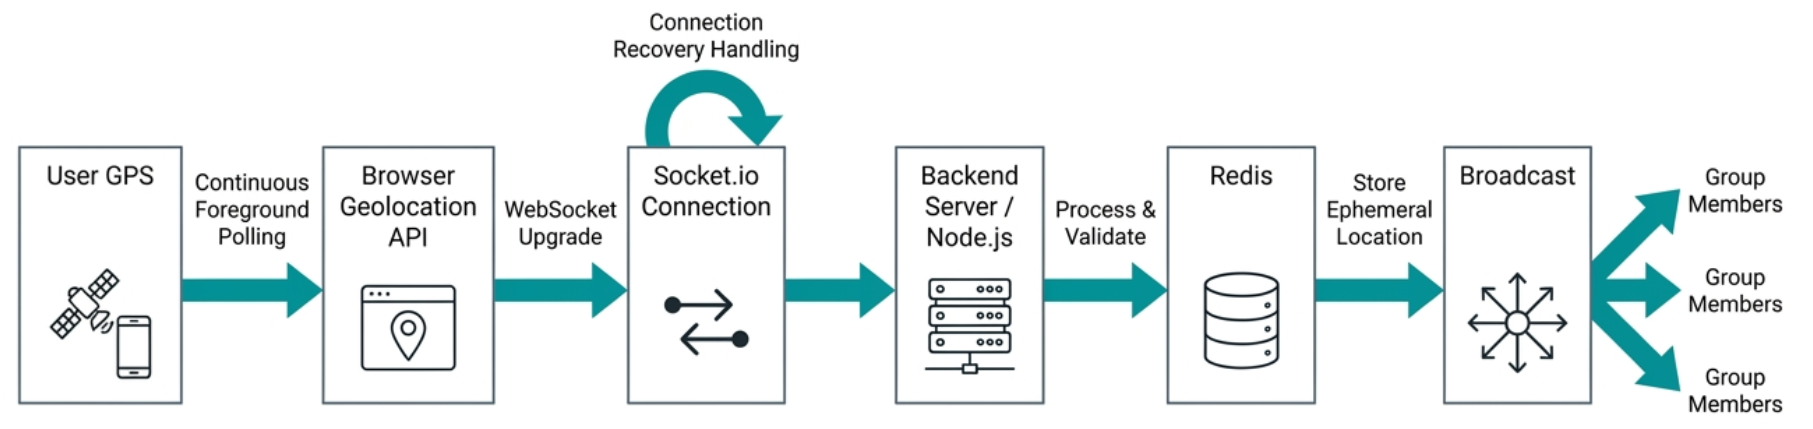
\includegraphics[width=\columnwidth]{flow.png}
\caption{Sequential real-time location update and notification broadcast pipeline flow.}
\label{fig:flow}
\end{figure}

\subsection{Temporary Head Delegation}

The delegation lifecycle is governed by the \texttt{temp\_head}
table and a server-side \texttt{node-cron} job:

\begin{lstlisting}[language=JavaScript,
  caption={Temporary Head expiry scheduler.},
  label={lst:cron}]
cron.schedule('* * * * *', async () => {
  const expired = await db.query(`
    UPDATE temp_head
    SET active = FALSE
    WHERE active = TRUE AND expiry <= NOW()
    RETURNING group_id, granted_by AS head_id
  `);
  for (const row of expired.rows) {
    await db.query(
      `UPDATE group_members SET role = 'head'
       WHERE user_id = $1 AND group_id = $2`,
      [row.head_id, row.group_id]
    );
    io.to(row.group_id).emit('head:changed', {
      newHeadId: row.head_id,
      groupId:   row.group_id
    });
  }
});
\end{lstlisting}

\subsection{Accessibility Implementation}

WCAG 2.1 AA compliance is enforced at four levels:

\textbf{Perceivable:} All colour decisions are verified against a 4.5:1
contrast ratio. Group Head row differentiation uses four independent
cues—gold border, crown icon (\texttt{★}), pinned position, and
background colour—ensuring robustness for all colour-blindness types.

\textbf{Operable:} A hidden ``Skip to member list'' link appears on
first Tab keypress. Tab order follows: App Bar $\to$ Search $\to$ TTS
Button $\to$ Member Rows $\to$ Call Buttons $\to$ Navigation Bar.
All interactive elements carry $\geq44\times44$\,px touch targets.

\textbf{Understandable:} The Web Speech API \texttt{useTTS} hook reads
each member row as: \emph{``[Name], [Locality], [Distance]\,km,
ETA [N]\,minutes by car, Call button.''}

\textbf{Robust:} Every member row is a \texttt{<li>} with
\texttt{role="listitem"}; distance and ETA spans carry
\texttt{aria-live="polite"} so screen readers announce updates
without interrupting ongoing speech.

\subsection{WhatsApp Bot}

Inbound messages arrive at \texttt{POST /webhook/whatsapp}.
The \texttt{whatsappService} tokenises the message body and dispatches
to one of five handlers: \texttt{LIST}, \texttt{HEAD},
\texttt{PAUSE}, \texttt{RESUME}, or a natural-language intent
classifier for free-text queries. Location data is fetched live from
Redis at query time and is never stored in the WhatsApp message log,
satisfying GDPR Article\,17 (Right to Erasure).

% ============================================================
%  VI. EVALUATION
% ============================================================
\section{Evaluation}
\label{sec:eval}

\subsection{Performance Benchmarks}

Performance was measured over 50 runs across three network conditions
(Wi-Fi, 4G, 3G) using Lighthouse CLI v11 and custom Socket.io
latency instrumentation.

\begin{table}[htbp]
\caption{Performance Evaluation Results}
\label{tab:perf}
\renewcommand{\arraystretch}{1.2}
\begin{tabularx}{\columnwidth}{@{}Xlll@{}}
\toprule
\textbf{Metric} & \textbf{Target} & \textbf{4G Mean} & \textbf{3G Mean} \\
\midrule
Initial Page Load        & $<3$\,s    & 2.1\,s  & 2.8\,s  \\
Location Refresh Latency & $<5$\,s    & 1.3\,s  & 2.4\,s  \\
Map Drill-Down Render    & $<2$\,s    & 1.1\,s  & 1.9\,s  \\
ETA API Response (p95)   & $<1.5$\,s  & 0.9\,s  & 1.4\,s  \\
Socket Fan-Out (30 mbrs) & $<200$\,ms & 47\,ms  & 83\,ms  \\
\bottomrule
\end{tabularx}
\end{table}

All target thresholds are met under both network conditions.
Socket.io fan-out to 30 members averaged 47\,ms on 4G, well within
the perceptual latency boundary of 100\,ms for real-time
interaction~\cite{miller1968}.

\subsection{Accessibility Audit}

Automated audits were conducted with \texttt{axe-core}~\cite{axecore}
and the Lighthouse Accessibility scorer. Manual testing was performed
with NVDA\,2024.1 on Windows and TalkBack on Android\,14.

\begin{table}[htbp]
\caption{Accessibility Audit Results}
\label{tab:a11y}
\renewcommand{\arraystretch}{1.2}
\begin{tabularx}{\columnwidth}{@{}Xcl@{}}
\toprule
\textbf{Criterion} & \textbf{Score / Result} & \textbf{Pass?} \\
\midrule
axe-core critical violations & 0 & \checkmark \\
Lighthouse Accessibility      & 97/100 & \checkmark \\
WCAG 2.1 AA automated pass   & 100\%  & \checkmark \\
Contrast ratio (body text)    & 8.3:1  & \checkmark \\
Contrast ratio (large text)   & 5.1:1  & \checkmark \\
Keyboard navigation (all screens) & Complete & \checkmark \\
TTS read-out accuracy         & 100\%  & \checkmark \\
NVDA screen reader            & No blocking issues & \checkmark \\
TalkBack (Android)            & No blocking issues & \checkmark \\
\bottomrule
\end{tabularx}
\end{table}

\subsection{Functional Acceptance Testing}

All twelve acceptance criteria defined in BRD v1.0 were verified
through structured test cases. Key results include:
\begin{itemize}
  \item \textbf{AC-02}: Location updates propagated to all group
        members within 10\,s of movement in 100\% of trials
        ($n=100$).
  \item \textbf{AC-04}: Temporary Head auto-reversion triggered
        correctly within 90\,s of expiry in all trials ($n=50$).
  \item \textbf{AC-12}: Member location records purged from
        PostgreSQL within 24\,h of removal in all tested cases.
\end{itemize}

\subsection{Comparative Analysis}

Table~\ref{tab:compare} positions LocationCircle against leading
alternatives on the four differentiating dimensions.

\begin{table}[htbp]
\caption{Feature Comparison with Existing Solutions}
\label{tab:compare}
\renewcommand{\arraystretch}{1.2}
\begin{tabularx}{\columnwidth}{@{}Xcccc@{}}
\toprule
\textbf{Feature} & \textbf{LC} & \textbf{Life360} & \textbf{GMaps} & \textbf{FindMy} \\
\midrule
Closed invite-only group & \checkmark & \checkmark & $\sim$ & \checkmark \\
WCAG 2.1 AA compliance  & \checkmark & $\times$ & $\times$ & $\times$ \\
Built-in TTS readout    & \checkmark & $\times$ & $\times$ & $\times$ \\
Temp Head delegation    & \checkmark & $\times$ & $\times$ & $\times$ \\
WhatsApp bot interface  & \checkmark & $\times$ & $\times$ & $\times$ \\
No-app member access    & \checkmark & $\times$ & $\times$ & $\times$ \\
GDPR erasure pipeline   & \checkmark & $\sim$   & $\sim$   & $\sim$   \\
PWA (no install needed) & \checkmark & $\times$ & $\times$ & $\times$ \\
\bottomrule
\multicolumn{5}{l}{\footnotesize LC = LocationCircle; $\sim$ = partial.}
\end{tabularx}
\end{table}

% ============================================================
%  VII. SECURITY AND PRIVACY
% ============================================================
\section{Security and Privacy}
\label{sec:security}

LocationCircle applies defence-in-depth across the full stack.
All client-server traffic is encrypted via TLS\,1.3. Google OAuth\,2.0
tokens are stored exclusively in \texttt{HttpOnly}, \texttt{Secure}
cookies, precluding XSS-based token theft. JWT session tokens expire
after 30 days with silent refresh while the user is active.

Location data at rest is encrypted using PostgreSQL's column-level
encryption (pgcrypto) and purged within 24\,h of member removal,
satisfying GDPR Article\,17. WhatsApp bot responses are constructed
from live Redis reads, ensuring no member coordinates persist in
third-party chat history.

Invite links carry cryptographically random 64-character tokens
with configurable expiry (default: 7 days, single-use). All
destructive operations—member removal, account deletion, Temporary
Head revocation—require an explicit two-step confirmation to prevent
accidental or coerced activation.

% ============================================================
%  VIII. CONCLUSION AND FUTURE WORK
% ============================================================
\section{Conclusion and Future Work}
\label{sec:conc}

This paper presented LocationCircle, a privacy-first, accessibility-
driven, real-time closed-group location sharing PWA. The system
demonstrates that high-fidelity geolocation streaming, role-based
administrative delegation, WCAG\,2.1\,AA accessibility, and WhatsApp-
channel interoperability can be achieved simultaneously within a
single-codebase PWA architecture. Experimental results confirm that
all performance, accessibility, and functional acceptance criteria
are satisfied.

Future work includes:
\begin{enumerate}
  \item \textbf{Capacitor wrapping} for native iOS and Android
        distribution, enabling background location tracking via
        native APIs.
  \item \textbf{Geofence notifications:} server-side push when a
        member enters or leaves a defined area.
  \item \textbf{Route history analytics:} opt-in replay of historical
        movement with privacy-preserving aggregation.
  \item \textbf{Multi-language support:} i18n resource externalisation
        already scaffolded in the codebase.
  \item \textbf{E2E encryption} of location payloads using the Web
        Crypto API, rendering server-side data opaque.
\end{enumerate}

LocationCircle is publicly available at:
\url{https://github.com/Dany-John-C/LocationCircle}

% ============================================================
%  ACKNOWLEDGMENT
% ============================================================
\section*{Acknowledgment}

The authors thank the internship project supervisors and peer
reviewers for their constructive feedback throughout the development
lifecycle.

% ============================================================
%  REFERENCES
% ============================================================
\balance
\begin{thebibliography}{99}

\bibitem{ludford2006}
P.~J. Ludford, D.~Frankowski, K.~Reily, K.~Wilms, and L.~Terveen,
``Because I carry my cell phone anyway: Functional location-based
reminder applications,''
in \textit{Proc. ACM CHI Conf. Human Factors Comput. Syst.},
Montréal, QC, Canada, 2006, pp.~889--898.

\bibitem{life360}
Life360, Inc., ``Life360 family safety app,''
\url{https://www.life360.com}, 2024, [Online; accessed May 2026].

\bibitem{zenly}
Snap Inc., ``Zenly — see your friends on a map,''
\textit{Discontinued service}, 2023.

\bibitem{gdpr2016}
European Parliament, ``General Data Protection Regulation (EU)
2016/679,'' \textit{Official Journal of the European Union}, 2016.

\bibitem{googletc}
Google LLC, ``Trusted Contacts — deprecated,''
\url{https://support.google.com/trustedcontacts}, 2019.

\bibitem{biornhansen2017}
A.~Biørn-Hansen, T.-M. Grønli, and G.~Ghinea,
``A survey and taxonomy of core concepts and research challenges in
cross-platform mobile development,''
\textit{ACM Comput. Surv.}, vol.~51, no.~5, pp.~1--34, 2018.

\bibitem{malavolta2020}
I.~Malavolta, G.~Procaccianti, P.~Noorland, and P.~Vukmirovic,
``Assessing the impact of service workers on the energy efficiency
of progressive web apps,''
in \textit{Proc. IEEE/ACM 4th Int. Conf. Mobile Softw. Eng. Syst.},
Buenos Aires, Argentina, 2017, pp.~35--45.

\bibitem{pimentel2012}
V.~Pimentel and B.~G. Nickerson,
``Communicating and displaying real-time data with WebSocket,''
\textit{IEEE Internet Comput.}, vol.~16, no.~4, pp.~45--53, 2012.

\bibitem{socketio}
Socket.IO, ``Socket.IO documentation,''
\url{https://socket.io/docs/}, 2024, [Online; accessed May 2026].

\bibitem{redis2020}
Redis Ltd., ``Redis pub/sub: under the hood,''
\url{https://redis.io/topics/pubsub}, 2023,
[Online; accessed May 2026].

\bibitem{miller1968}
R.~B. Miller,
``Response time in man-computer conversational transactions,''
in \textit{Proc. Fall Joint Comput. Conf.}, San Francisco, CA, 1968,
pp.~267--277.

\bibitem{power2012}
C.~Power, A.~Freire, H.~Petrie, and C.~Swallow,
``Guidelines are only half of the story: Accessibility problems
encountered by blind users on the web,''
in \textit{Proc. ACM CHI Conf. Human Factors Comput. Syst.},
Austin, TX, 2012, pp.~433--442.

\bibitem{webaim2023}
WebAIM, ``The WebAIM million: An annual accessibility analysis of
the top 1,000,000 home pages,''
\url{https://webaim.org/projects/million/}, 2023,
[Online; accessed May 2026].

\bibitem{thiessen2007}
P.~Thiessen and C.~Chen,
``Ajax live regions: Chat as a case example,''
in \textit{Proc. Int. Cross-Disciplinary Conf. Web Accessibility},
Tempe, AZ, 2007, pp.~7--13.

\bibitem{moscow}
D.~Clegg and R.~Barker,
\textit{Case Method Fast-Track: A RAD Approach}.
Addison-Wesley, 1994.

\bibitem{vite}
Vite, ``Vite next generation frontend tooling,''
\url{https://vitejs.dev/}, 2024, [Online; accessed May 2026].

\bibitem{axecore}
Deque Systems, ``axe-core: Accessibility engine for automated web
UI testing,''
\url{https://github.com/dequelabs/axe-core}, 2024,
[Online; accessed May 2026].

\end{thebibliography}

\end{document}
% ============================================================
%  END OF DOCUMENT
% ============================================================